\chapter{Requerimientos}
\section{Analisis de requerimientos}
�Cu\'al es la finalidad de esta actividad dentro de la empresa?
\\%
\\%
Garantizar que el Sistema Administre todos los procesos de la organizaci\'on y asi generar un mejor funcionamiento y control en la panader\'ia.
\\%
\\%
�Qu\'e pasos se siguen para llevarla a cabo?
\\%
\\%
Software el cual llevara toda la administraci\'on de transacciones, ventas y compra de productos de una panader\'ia la cual se tendr\'a registrada en una base de datos lo que ayudara a generar reportes.
\\%
\\%
�D\'onde se realizan estos pasos?
\\%
\\%
Los pasos a efectuar se empiezan a realizar en la parte de compra de insumos que es donde empieza a generar los procesos y all\'i poder implementar este sistema de administraci\'on y gestionara todos los procesos hasta la entrega del producto.
\\%
\\%
�Qui\'enes los realizan?
\\%
\\%
Hay tres departamentos los cuales son los cuales tienen los principales procesos de producci\'on que son: inventarios de insumo, Producci\'on e inventarios de producci\'on, de estos tres departamentos podemos ver todos los procesos que se realizan dentro de la organizaci\'on.
\\%
\\%
�Cu\'anto tiempo tardan en efectuarlos?
\\%
\\%
Al tener los datos de cada proceso como por ejemplo en los inventarios de insumos al tomar todos los datos la respuesta es inmediata generando reportes e informaci\'on necesaria para la producci\'on.
\\%
\\%
�Con cuanta frecuencia lo hacen?
\\%
\\%
La Gesti\'on de informaci\'on estar\'a actualizada siempre que se ingresen datos a los registros de informaci\'on de la panader\'ia esto permite tener un control inmediato de cualquier informaci\'on err\'onea.
\\%
\\%
�Qui\'enes emplean la informaci\'on resultante?
\\%
\\%
Administrador de la panader\'ia el cual llevara el reporte diario de los movimientos empleados en la panader\'ia.%
\section{Analisis de requerimientos}
\subsection{Requerimientos generales}
\\%
\\%
�Qu\'e es lo que se hace?
\\%
\\%
Administrar todos los procesos de la organizaci\'on para generar controles y rapidez en efectuar los procesos.
\\%
\\%
�C\'omo se hace?
\\%
\\%
Por medio de un software el cual esta adecuado para poder administrar los procesos, como los inventarios de insumo que el administrara dichos productos y tendr� el debido control para no tener perdida de informaci\'on y tener informaci\'on necesaria al instante.
\\%
\\%
�Con que frecuencia se realiza?
\\%
\\%
Se realiza diariamente ya que es un sistema de administraci\'on de procesos y los procesos se est\'an efectuando diariamente.
\\%
\\%
�Qu\'e tan grande es el volumen de las transacciones?
\\%
\\%
Las transacciones dependen del tipo de sucursal. Pero en si todas tiene grandes volumen de transacciones por ello vamos a implementar este sistema.
\\%
\\%
�Cu\'al es el grado de eficiencia con el que se efect\'uan las tareas?
\\%
\\%
Definir\'iamos como alta aunque quedar\'ia muy robusto por la calidad de datos que ingresara cada departamento de la organizaci\'on y su base de datos la cual se actualizara con cada informaci\'on nueva obtenida. El software tendr\'a un alto desempe�o con espuestas inmediatas y f\'acil control de consultas.
\\%
\\%
\subsection{Requerimientos b\'asicos}
�Cu\'al es el proceso b\'asico de la empresa?
\\%
\\%
El proceso b\'asico de la empresa es la producci\'on para el cual implementaremos el software de administraci\'on de procesos.
\\%
\\%
�Qu\'e datos utiliza o produce este proceso?
\\%
\\%
Este proceso genera muchos datos ya que al realizarse una producci\'on obtenemos datos de insumos y de productos ya producidos, y as\'i como tal informaci\'on de productos que fueron mal producidos e inservibles.
\\%
\\%
�Qu\'e controles de desempe\~no utiliza?
\\%
\\%
Seguimiento diario por el administrador. El cual observara  los procesos de la panaderia y de la misma forma  el funcionamiento del software.
\section{Requerimientos funcionales}
\begin{figure}[htbp]
%centering es para centrar la imagen
	\centering
%aca es donde se incluye la imagen, se da el ancho(width), \textwidth significa que con repescto al tamano del
%texto y luego la ruta, relativa siempre es decir, a partir de donde se esta, como images esta ahi
%dentro, solo se usa desde images y ojala nada de espacios en el nombre de la imagen
		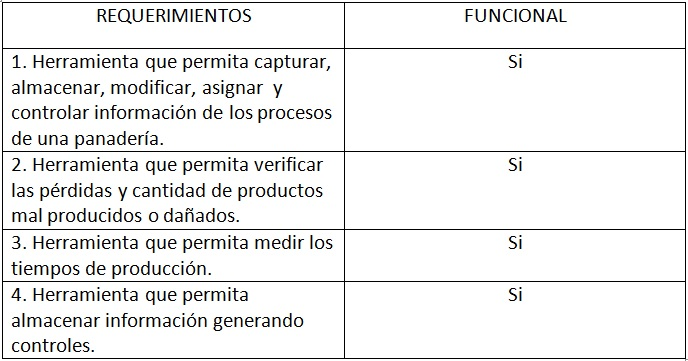
\includegraphics[width=0.60\textwidth]{images/requerimientosfuncionales.jpg}
%el caption es para el texto que aparece debajo de la imagen
	\caption{Requerimientos funcionales}
%label es para darle una referencia, por ejemplo si uno dice "como se puede ver en la imagen a1"
	\label{fig:Requerimientos funcionales}
\end{figure}%
\\%
\\%
Requerimientos no funcionales
\\%
\begin{figure}[htbp]
%centering es para centrar la imagen
	\centering
%aca es donde se incluye la imagen, se da el ancho(width), \textwidth significa que con repescto al tamano del
%texto y luego la ruta, relativa siempre es decir, a partir de donde se esta, como images esta ahi
%dentro, solo se usa desde images y ojala nada de espacios en el nombre de la imagen
		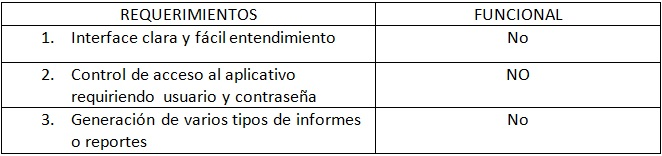
\includegraphics[width=0.60\textwidth]{images/requerimientosnofuncionales.jpg}
%el caption es para el texto que aparece debajo de la imagen
	\caption{Requerimientos no funcionales}
%label es para darle una referencia, por ejemplo si uno dice "como se puede ver en la imagen a1"
	\label{fig:Requerimientos no funcionales}
\end{figure}%
\\%
\\%
\\%
\section{Priorizar los requerimientos del sistema}
Por medio de la siguiente tabla se da muestra del  nivel de prioridad de los requerimientos que principalmente se tendr\'an en cuenta para el dise\~no del sistema.
\\%
\begin{figure}[htbp]
%centering es para centrar la imagen
	\centering
%aca es donde se incluye la imagen, se da el ancho(width), \textwidth significa que con repescto al tamano del
%texto y luego la ruta, relativa siempre es decir, a partir de donde se esta, como images esta ahi
%dentro, solo se usa desde images y ojala nada de espacios en el nombre de la imagen
		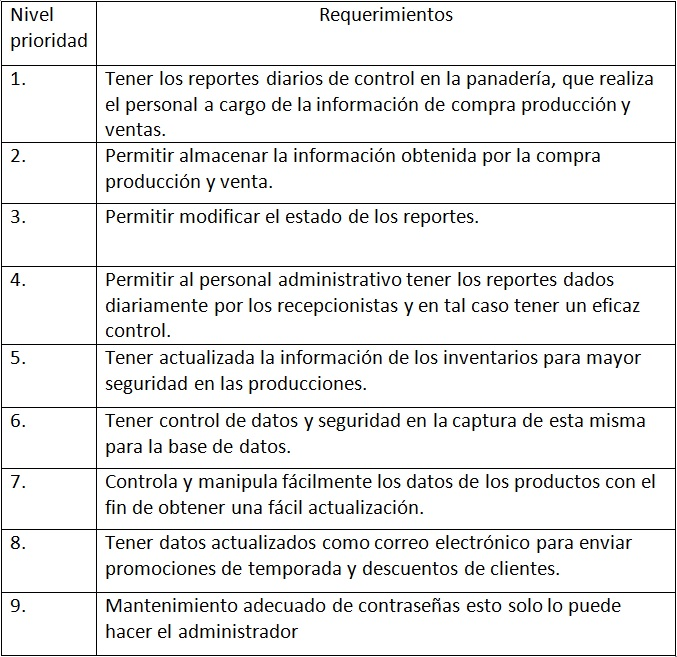
\includegraphics[width=0.60\textwidth]{images/requerimientos.jpg}
%el caption es para el texto que aparece debajo de la imagen
	\caption{Requerimientos}
%label es para darle una referencia, por ejemplo si uno dice "como se puede ver en la imagen a1"
	\label{fig:Requerimientos}
\end{figure}%
